\documentclass[border=10pt]{standalone}
\usepackage{tikz}
\usetikzlibrary{arrows.meta, shapes.geometric}

\begin{document}
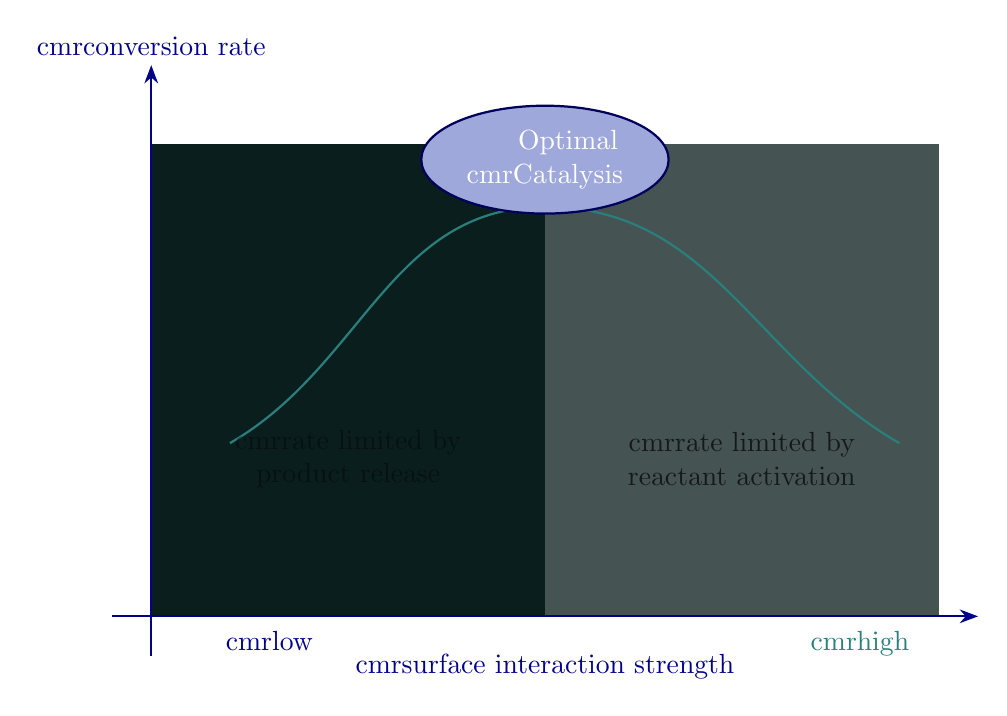
\begin{tikzpicture}[
    font=\familydefault, % Default LaTeX serif font
    axis/.style={-Stealth, thick, color=axisblue},
    label/.style={color=axisblue},
    volcano/.style={thick, color=plotgreen},
    oval_node/.style={
        ellipse,
        draw=ovalborder,
        fill=ovalfill,
        text=white,
        align=center,
        minimum height=1.1cm,
        minimum width=2.8cm,
        thick
    },
    region_text/.style={
        text=black,
        text width=3.5cm,
        align=center
    }
]

% Define colors based on the image
\definecolor{axisblue}{HTML}{00008B}
\definecolor{plotgreen}{HTML}{2A7F7C}
\definecolor{bgleft}{HTML}{0B1E1E}
\definecolor{bgright}{HTML}{455353}
\definecolor{ovalfill}{HTML}{9FA8DA}
\definecolor{ovalborder}{HTML}{00005A}

% Define key coordinates and dimensions
\def\xmax{10}
\def\ymax{6}
\def\xpeak{5}
\def\ypeak{5.2}
\def\yoval{5.8}

% 1. Draw the background regions
\fill[bgleft] (0,0) rectangle (\xpeak, \ymax);
\fill[bgright] (\xpeak,0) rectangle (\xmax, \ymax);

% 2. Draw the volcano plot line
\draw[volcano] (1, 2.2) to[out=30, in=180] (\xpeak, \ypeak) to[out=0, in=150] (9.5, 2.2);

% 3. Draw the axes
\draw[axis] (-0.5, 0) -- (\xmax + 0.5, 0);
\draw[axis] (0, -0.5) -- (0, \ymax + 1);

% 4. Add axis labels and markers
\node[label, above] at (0, \ymax + 1) {conversion rate};
\node[label, below=10pt] at (\xpeak, 0) {surface interaction strength};
\node[label, below=2pt] at (1.5, 0) {low};
\node[color=plotgreen, below=2pt] at (9, 0) {high};

% 5. Add text inside the regions with opacity for low contrast
\node[region_text, opacity=0.4] at (2.5, 2) {rate limited by\\product release};
\node[region_text, opacity=0.7] at (7.5, 2) {rate limited by\\reactant activation};

% 6. Add the "Optimal Catalysis" ellipse node
\node[oval_node] at (\xpeak, \yoval) {Optimal \\ Catalysis};

\end{tikzpicture}
\end{document}